El faraón cobraba impuestos directamente proporcionales al tamaño de la tierra. Eso generó algunos conocimientos matemáticos: proporción, que estaba sujeta a cambios, por ejemplo si desbordaba el nilo, la cantidad de tierra cosechada era menor por lo tanto había que pagar menos. Y por el caso contrario si un terreno bien sedimentado producía una buena cosecha, se pagaba más. Por lo que había que estar constantemente midiendo tierras. 
Tenían un sistema de numeración, era no posicional. Y también unidades de medida para longitudes, superficies. Las unidades correspondían a las medidas del faraón. Palmo, codo, pie. Esto traía problemas porque a veces los faraones eran niños, o si cambiaba el faraón, cambiaba el patrón de unidad. Luego crean medidas estándar (que habrán provenido de algún faraón) que se mantuvieron constantes. 

Los impuestos se pagaban con semillas. Para saber cuánto pagar, necesitaban unidades de capacidad. Tenían vasijas de distintos tamaños, unas múltiplos de las otras.

Necesitaban alguna especie de calendario para contar con alguna manera de predecir las crecidas del Nilo. 

Tenían una cuerda de 12 nudos para medir ángulos rectos, esto directamente relacionado con la necesidad de parcelar las tierras para la agricultura. Por ejemplo, si tengo una cuerda con 12 nudos y los dispongo en lados imaginarios compuestos por 3, 4 y 5 nudos tengo triángulo rectángulo, un triángulo que verifica el teorema de pitágoras. Había egipcios que tenían como trabajo medir ángulos rectos: eran los tendedores de cuerdas. De esta manera descubrieron que 3, 4 y 5 es lo que llamamos una terna pitagórica: números que verifican el teorema de pitágoras. Y descubrieron propiedades al respecto: que si a cada número lo multiplicaban por otro número, seguía siendo una terna pitagórica.

El sistema de numeración es un sistema no posicional que permitía representar enteros no positivos y también números racionales positivos. No existen los números negativos para ellos y tampoco tienen cero. 
\\[0.5cm]
        \begin{minipage}{0.2\textwidth}
            \begin{flushleft} 
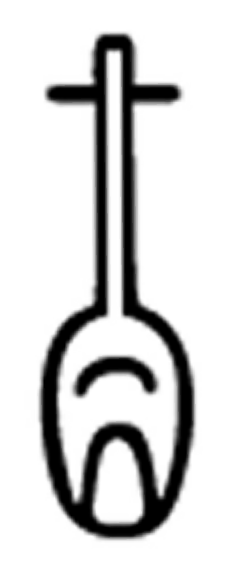
\includegraphics[scale=0.2]{20160804_080346.png}
            \end{flushleft}
        \end{minipage}
        ~
        \begin{minipage}{0.74\textwidth}

A pesar de no tener un cero, tenían un protocero, "nfr". Tiene algunas características del cero pero no simboliza la nada. El símbolo se encontraba en las pirámides, dispuesto de forma tal que extendido hacía fuera de la pirámide marcaba el nivel del suelo. Del cero para abajo hay tierra, del cero para arriba hay aire. Es como una especia de nivel, un origen de coordenadas. Pero no solo se encontraba en las pirámides. En los libros contables del faraón aparecía cuando estaba equilibrado el saldo a favor y el saldo en contra. Simbolicamente representa la belleza y el equilibrio.

        \end{minipage}\\[0.5cm]

Aunque para los sistemas no posicionales es difícil hacer algoritmos, ellos desarrollan un algoritmo de multiplicación que involucra propiedades asociativas, distributivas. 

Resolvían problemas de geometría del espacio: el volumen de una pirámide, áreas laterales de la pirámide; también volumen de una semiesfera para saber el volumen de unas cestas que tenían, también la superficie de la semiesfera, para saber la superficie que tenían que tejer. Trabajaron también con círculos, calculaban área y longitud de la circunferencia. Utilizaron varios valores para pi, pero el que más usaban era 22/7 (3,1428, bastante aproximado). 

Resolvían ecuaciones de 1er y 2do grado, y si bien tenían algoritmos para multiplicación y suma, tenían las operaciones tabuladas. Era mucho más rápido mirar en una tabla que hacer cuentas. También tenían concepto de sucesiones y series como concepto de sumas repetidas, no llegaban al infinito (no lo manejaban conceptualmente) pero si tenían la noción de poder ir agregando términos. No se plantean su naturaleza de entero o racional o si la suma sucesiva tiende a algo, es algo mucho más concreto (es una cultura empírica, no tiene demostraciones. para que algo este bien basta con que la práctica lo corrobore).







